\documentclass{article}
\usepackage{graphicx, float} % Required for inserting images
\usepackage{enumitem,amssymb,amsmath}
\usepackage{fullpage}
\usepackage{multicol}
\usepackage{hyperref}
\usepackage{caption, subcaption}

\usepackage[style=authoryear,sorting=nyt,maxnames=1,maxcitenames=1,minnames=1,backend=biber]{biblatex}
\addbibresource{biblatex/WaterConnectivity.bib}
\addbibresource{biblatex/code.bib}

% Setup of hyperlinks incompilation
\usepackage{hyperref}
\hypersetup{colorlinks=true,allcolors=black}
\usepackage{hypcap}

\numberwithin{equation}{section}


\title{Relation Between Biomass Patterns and Water Flux in an Arid Drainage Basin System}

\author{Yotam Ohad \and Prof. Ehud Meron}

\begin{document}

\maketitle

\begin{abstract}
    In this study, we investigate the relationship between water flux emanating from a drainage basin and the patterns formed by its vegetation. Our findings align with previous research \parencite[]{meron_vegetation_2004} on the correlation between vegetation patterns and water availability. Furthermore, we propose a methodology to associate vegetation patterns with outward waterflux.
\end{abstract}

\section{Introduction}
In dryland ecosystem studies, the fundamental unit of consideration is the drainage basin \parencite{yair_case_1982}.
The drainage basin has two main components: the slope and the riverbed downhill, which is commonly a dry riverbed. The biomass ratio between the slope and the riverbed has not yet been the subject of studies addressing the effects of climate change and severe droughts on vegetation (corroborated by Prof. Moshe Shachak). This ratio depends to a large extent on the patchy nature of the vegetation that develops on the slope, which tends to self-organizes in nearly periodic patterns for nearly homogeneous slopes (\cite{lefever_origin_1997}, \cite{valentin_soil_1999}, \cite{klausmeier_regular_1999}, \cite{von_hardenberg_diversity_2001}).

A commonly observed vegetation pattern on slopped terrains is banded vegetation consisting of alternating stripes of vegetation and bare soil, oriented perpendicular to the slope direction. In this configuration each stripe benefits not only from direct rainfall but also from the interception of runoff water generated in the bare-soil stripe uphill, where the infiltration rate of surface water into the soil is lower than the rate in the vegetation stripe \parencite{meron_vegetation_2019}. However, at sufficiently lower precipitation rates vegetation stripes break into arc-shaped vegetation spots and concomitantly bare-soil areas merge to form longer pathways for water flow downhill. These pathways, in turn, increase the seepage of water and nutrients from the slope to the riverbed and change the ratio of vegetation biomass between the two components. Longer pathways of water and nutrient flow are often described as increased connectivity \parencite{okin_connectivity_2015}

\section{The Model}
\subsection{Model's Equations}
We will investigate the issue of biomass patterns in drainage basins using the model proposed by \cite{gilad_phys_2004}, and \cite{gilad_mathematical_2007}. We choose this model as, unlike simpler models, it makes a distinction between soil water and surface water. Therefore distinguishing the surface water from the rest of the system, enabling us to examine it and the water flux which derives from it.

The model can be written in a non-dimensional form as such:
\begin{align}
    \partial_t b & = G_b(x,y) b(1-b) - b + \delta_b\nabla^2 b              \\
    \partial_t w & = Ih - \nu(1-\rho b)w - G_w(x,y)w + \delta_w \nabla^2 w \\
    \partial_t h & = p - Ih - \nabla \cdot \vec{J}
\end{align}
where $b(x,y),w(x,y),h(x,y)$ are the non-dimensional functions from $\mathbb{R}^2$ to $\mathbb{R}$ describing the biomass, soil water, and surface water. $\vec{J}$ is the (non-dimensional) water flux and is given by:
\begin{align}
    \label{eq:flux_def}
    \vec{J} =  -2\delta_h h\nabla\left(h+\zeta(x,y)\right)
\end{align}
using $\zeta$ as the topography function of the slope. Assuming uniform slope $\zeta(x,y)=my$, the water flux can be written as:
\begin{equation}
    \nabla \cdot \vec{J} = -\delta_h \nabla^2(h^2) - 2\delta_h m \partial_y h
\end{equation}
$I$ is the infiltration rate and is defined using
\begin{equation}
    I = \alpha \frac{b+qf}{b+q}
\end{equation}
This form captures the dependence of the infiltration rate on the biomass. $f\in[0,1]$ and $q\in(0,\infty)$, so for large values of $f$ (close to 1), the infiltration rate doesn't depends much on the biomass, while for small values of $f$ (close to 0) the dependence is extremely large, i.e., $I\approx \alpha\frac{b}{b+q}$.

The Functions $G_b,G_w$ are defined using the kernel function
\begin{equation}
    g(\mathbf{x}, \mathbf{x'},t) = \frac{1}{2\pi} \exp\left[-\frac{\left|\mathbf{x}-\mathbf{x'}\right|^2}{2(1+\eta b(\mathbf{x},t))^2}\right]
\end{equation} as \begin{align}
    G_b(\mathbf{x},t) & = \nu \int_\Omega g(\mathbf{x},\mathbf{x'},t)w(\mathbf{x'},t)d\mathbf{x'}    \\
    G_w(\mathbf{x},t) & = \gamma \int_\Omega g(\mathbf{x'},\mathbf{x},t)b(\mathbf{x'},t)d\mathbf{x'}
\end{align}
We add the assumption the the root zone is narrowly confined. In the dimensional form this means that $S_0\rightarrow 0$ \parencite[see][eq (3)]{gilad_phys_2004}. Using this assumption we get:
\begin{align}
    G_b & = \nu w (1+\eta b)^2   \\
    G_w & = \gamma b(1+\eta b)^2
\end{align}
Our model equations are then:
\begin{align}
    \partial_t b & = \nu bw(1-b)(1+\eta b)^2 - b + \delta_b\nabla^2 b                   \\
    \partial_t w & = I h - \nu(1-\rho b)w - \gamma bw(1+\eta b)^2 + \delta_w \nabla^2 w \\
    \partial_t h & = p - I h - \nabla \cdot \vec{J}
\end{align}

\subsection{Scales of the slope}
From equation \ref{eq:flux_def}, assuming uniform slope, we can write the time derivative of $h$ in the following manner:
\begin{equation}
    \partial_t h = \frac{1}{1 - 2\delta_h m h} \left(p - I h + 2\delta_h h\nabla h\right)
\end{equation}
From this, we can see that if $0 < 2\delta_h m h \ll 1$ then the system dynamics do not depend on the terrain's slope.
In the next section, we'll use $\delta_h=0.01$ (see table \ref{table:constants_tables}).
The slopes will be in the range of $m\in[0,1]$ (up to $45^\circ$) and the values of $h$ will be in the range of $h\in[0,1]$.
Thus, we expect the dynamics in the simulations to not depend strongly on the slope.

\subsection{Uniform Bare Steady State Solution}
To be able to verify that our simulation indeed represents the mathematical model correctly, we derive in this section the linear stability of the uniform bare steady state solution. This linear stability can then be checked in the simulation.

\subsubsection{Solutions of the Model}
The uniform bare steady state solution of the model is a solution that has no vegetation at all, and homogeneous surface and soil water. In equation form we can write this as:
\begin{align}
    b(x,y)                      & =0  \\
    \partial_t w = \partial_t h & = 0 \\
    \nabla w = \nabla h         & = 0
\end{align}
From the first condition, we can see that both $\partial_tb=0$ and $\nabla b=0$ holds. We are left with the following system of equations:
\begin{align}
    0 & = \alpha h - \nu w \\
    0 & = p-\alpha f h
\end{align}
which admits the following solutions:
\begin{align}
    w_0 & = \frac{p}{\nu}      \\
    h_0 & = \frac{p}{\alpha f}
\end{align}
\subsubsection{Linear Stability Analysis}
We start by writing the right hand side of the model equations in operator form and equating it to zero to find the steady state.
\begin{align}\label{eqn:functional_eq}
    \vec{0}=\vec{F}[b,w,h]
\end{align}
To find the linear stability of the uniform bare steady state solution, we'll calculate the linear approximation of $\vec{F}$  when perturbing the solution we found using $\begin{bmatrix}\varepsilon_b(t) & \varepsilon_w(t) & \varepsilon_h(t)\end{bmatrix}^T e^{i\vec{k}\cdot\vec{r}}$, an infinitesimal perturbations with $0<|\varepsilon_s|\ll1$ for $s\in \{b,w,h\}$.  $\vec{r}=(x,y)$ is the position vector in the region, and $\vec{k}=(k_x,k_y)$ is the vector wave number of the perturbation.

Plugging this form into \ref{eqn:functional_eq}, we get the following relations:
\begin{align}
    \partial_t \varepsilon_b & = (-\delta_b k^2+p - 1)\varepsilon_b + o(\varepsilon^2)   \label{eq:eps_b}                                   \\
    \partial_t \varepsilon_w & = \frac{p}{q}(1-f)\varepsilon_b + (-\delta_wk^2-\nu)\varepsilon_w +\alpha f\varepsilon_h + o(\varepsilon^2)  \\
    \partial_t \varepsilon_h & = (-\alpha -2\delta_h \frac{p}{\alpha} k^2 +2i\delta_hk_ym) \varepsilon_h + o(\varepsilon^2)\label{eq:eps_h}
\end{align}
where $o(\varepsilon^2)$ are nonlinear terms in $\varepsilon_{b,w,h}$. We assume the initial perturbations are infinitesimal, so we can ignore nonlinear terms in \ref{eq:eps_b}-\ref{eq:eps_h}. We are left with the following linear ODE:
\begin{equation}
    \partial_t \begin{bmatrix}
        \varepsilon_b \\ \varepsilon_w \\ \varepsilon_h
    \end{bmatrix} = \begin{bmatrix}
        -\delta_b k^2+p - 1 & 0                & 0                                                       \\
        \frac{p}{q}(1-f)    & -\delta_wk^2-\nu & \alpha f                                                \\
        0                   & 0                & -\alpha -2\delta_h \frac{p}{\alpha} k^2 +2i\delta_hk_ym
    \end{bmatrix} \begin{bmatrix}
        \varepsilon_b \\ \varepsilon_w \\ \varepsilon_h
    \end{bmatrix}
\end{equation}
Solutions of these equation are linear combinations of the eigenvectors of the matrix. Each eigenvector grows if its eigenvalue is positive, and decays for negative eigenvalues. Linearly stable states would have all the eigenvalues as  negative. In this problem, the eigenvalues can be easily found to be:
\begin{align}
    \sigma_1 & = -\delta_b k^2+p - 1 \label{eq:sigma1}                   \\
    \sigma_2 & = -\delta_w k^2 -\nu                                      \\
    \sigma_3 & = -\alpha -2\delta_h \frac{p}{\alpha} k^2 +2i\delta_hk_ym
\end{align}
We see that the real parts of $\sigma_2,\sigma_3$ are negative for all $k^2 = k_x^2+k_y^2>0$.
For \ref{eq:sigma1}, to find the critical precipitation where the uniform zero vegetation loses stability we need to solve the following system:
\begin{align}
    \sigma_1             & = 0  \\
    \frac{d\sigma_1}{dk} & =  0
\end{align}
The second equation gives $k=0$ which then leads to $p_c=1$ (a local maximum of $\sigma_1)$. For $p<p_c$ then, the perturbations decrease while for $p>p_c$ the perturbations grow, changing the state of the system into a non-zero biomass state.
In the next section, we'll simulate the system slightly above and below $p_c$ to verify that the simulations indeed agree with the linear stability analysis.
We note here that the slope, in the case of linear terrain, only appears in the complex part of the eigenvalues and thus doesn't effect the linear stability. Its meaning comes into play only when the system is non-homogeneous. In this case, it relates to the speed at which spatial perturbation travel up the slope.

\section{Simulating the model}
We utilized the Python package, Dedalus3 \parencite[]{dedalus2020}, for the numerical simulations of the model. The code used in this paper, and scripts to generate the data used, can be found at \cite{Ohad_Relation_Between_Biomass_2023}.

\subsection{Boundary Conditions}
We now move to discuss how to simulate the model. For simplicity we choose a square region of $N\times N$ points, relating to an area of  $L\times L$  we wish to simulate. For the $x$ coordinates, we have periodic boundary conditions. For the $y$ axis, we wish to not force the total flux coming out of the region. This leads as to consider Neumann boundary condition at the bottom edge for the flux. Using $h(x,y=0)=h$ we can write $J_y=-2\delta_h h \frac{\partial}{\partial y}(h+\zeta)$ as the $y$ compononent of the flux. We can then write the boundary condition as:
\begin{equation}
    \frac{\partial J_y}{\partial y}(y=0) = 0
\end{equation}
or in terms of $h$:
\begin{equation}
    \left(\frac{\partial h}{\partial y}\right)^2 + h \frac{\partial^2 h}{\partial y^2} + m \frac{\partial h}{\partial y} = 0
\end{equation}

Using $H=\frac{\partial h}{\partial y}$ we can get a Neumann boundary condition for $h$, i.e., $\frac{\partial h}{\partial y}=A\in \mathbb{R}$.
\begin{align}
    \left(H + m + h\frac{\partial}{\partial y}\right)H         & = 0             \\
    \Rightarrow \frac{1}{H(H+m)} \frac{\partial H}{\partial y} & = - \frac{1}{h}
\end{align}
Integrating both sides over the range of $y$ values we get:
\begin{equation}
    \frac{1}{m}\ln{\frac{H}{H+m}} = -\int_0^{L_y} \frac{dy}{h}
\end{equation}
We can isolate $H$
\begin{equation}
    \frac{\partial h}{\partial y} (y=0) = H = m \frac{e^{-m \int_0^{L_y} \frac{dy}{h}}}{1 - e^{-m \int_0^{L_y} \frac{dy}{h}}}
\end{equation}

For other fields and edges in the $y$ coordinate, we chose a zero Neumann boundary condition - $\frac{\partial f}{\partial y}=0$.
Note that this additional condition makes the flux at the top edge equals to $mh$.
This means our top edge isn't the separation line between drainage basins, but rather a vertical segment of the drainage basin.

\subsection{Results}
The values of the constants of the non-dimensional model were taken from \parencite[]{gilad_mathematical_2007}.
The values used are shown in Table  \ref{table:constants_tables}.
\begin{table}[!ht]
    \centering
    \begin{tabular}{||cc||}
        \hline
        constant   & value          \\
        \hline\hline
        $m$        & $[0, 1]$       \\
        $p$        & $[0.9, 1.5]$   \\
        $\nu$      & $\frac{10}{3}$ \\
        $\eta$     & $3.5$          \\
        $\rho$     & $0.95$         \\
        $\gamma$   & $\frac{50}{3}$ \\
        $\alpha$   & $0.1$          \\
        $q$        & $0.05$         \\
        $f$        & $0.01$         \\
        $\delta_b$ & $\frac{1}{30}$ \\
        $\delta_w$ & $\frac{10}{3}$ \\
        $\delta_h$ & $0.01$         \\
        \hline
    \end{tabular}
    \caption{Values of simulation's constants.}
    \label{table:constants_tables}
\end{table}

Initially, we verified that the numerical simulation accurately reproduces the linear stability analysis.
The simulation started from the uniform zero biomass state, and was left to run for 500 years.
The precipitation values where chosen to be around $p_c$.
Figure \ref{fig:critical_point} shows the results of the simulation. We see that for $p<p_c$ the system decays to the zero biomass state, while for $p>p_c$ the system moves to a vegetation state. This is in agreement with the linear stability analysis. Below $p_c$ the perturbations decay, while above $p_c$ they grow.
\begin{figure}[!ht]
    \centering
    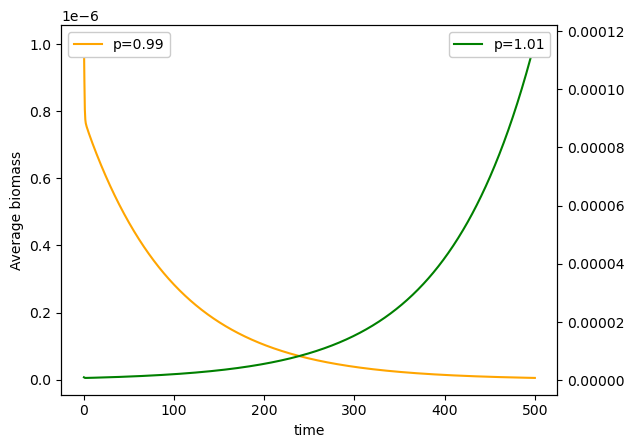
\includegraphics[scale=0.5]{plots/critical point.png}
    \caption{Simulations around $p_c$ (different scales)}
    \label{fig:critical_point}
\end{figure}

We now move to study the water flux in the system in the case of $p>p_c$.
We started each simulation from the uniform vegetation state, where the initial biomass was chosen to be $b=0.2$.
This value was used as it is higher than the biomass of the uniform vegetation state in our range of values of $p$, and thus the system will move to the patterned state.
We let the simulation run for 500-2000 years (until the uniform non-zero vegetation state lost stability), and plotted the flux going out of the region.
We simulated different slopes (figure \ref{fig:flux_out_slopes}) and different precipitation values (figure \ref{fig:flux_out_precipitation}).
In the begining of the simulations, there was a transitive state of lower outward flux, which was caused by the initial conditions of the simulation, and thus not added to the plots.

\begin{figure}[ht!]
    \centering
    \begin{subfigure}{.4\linewidth}
        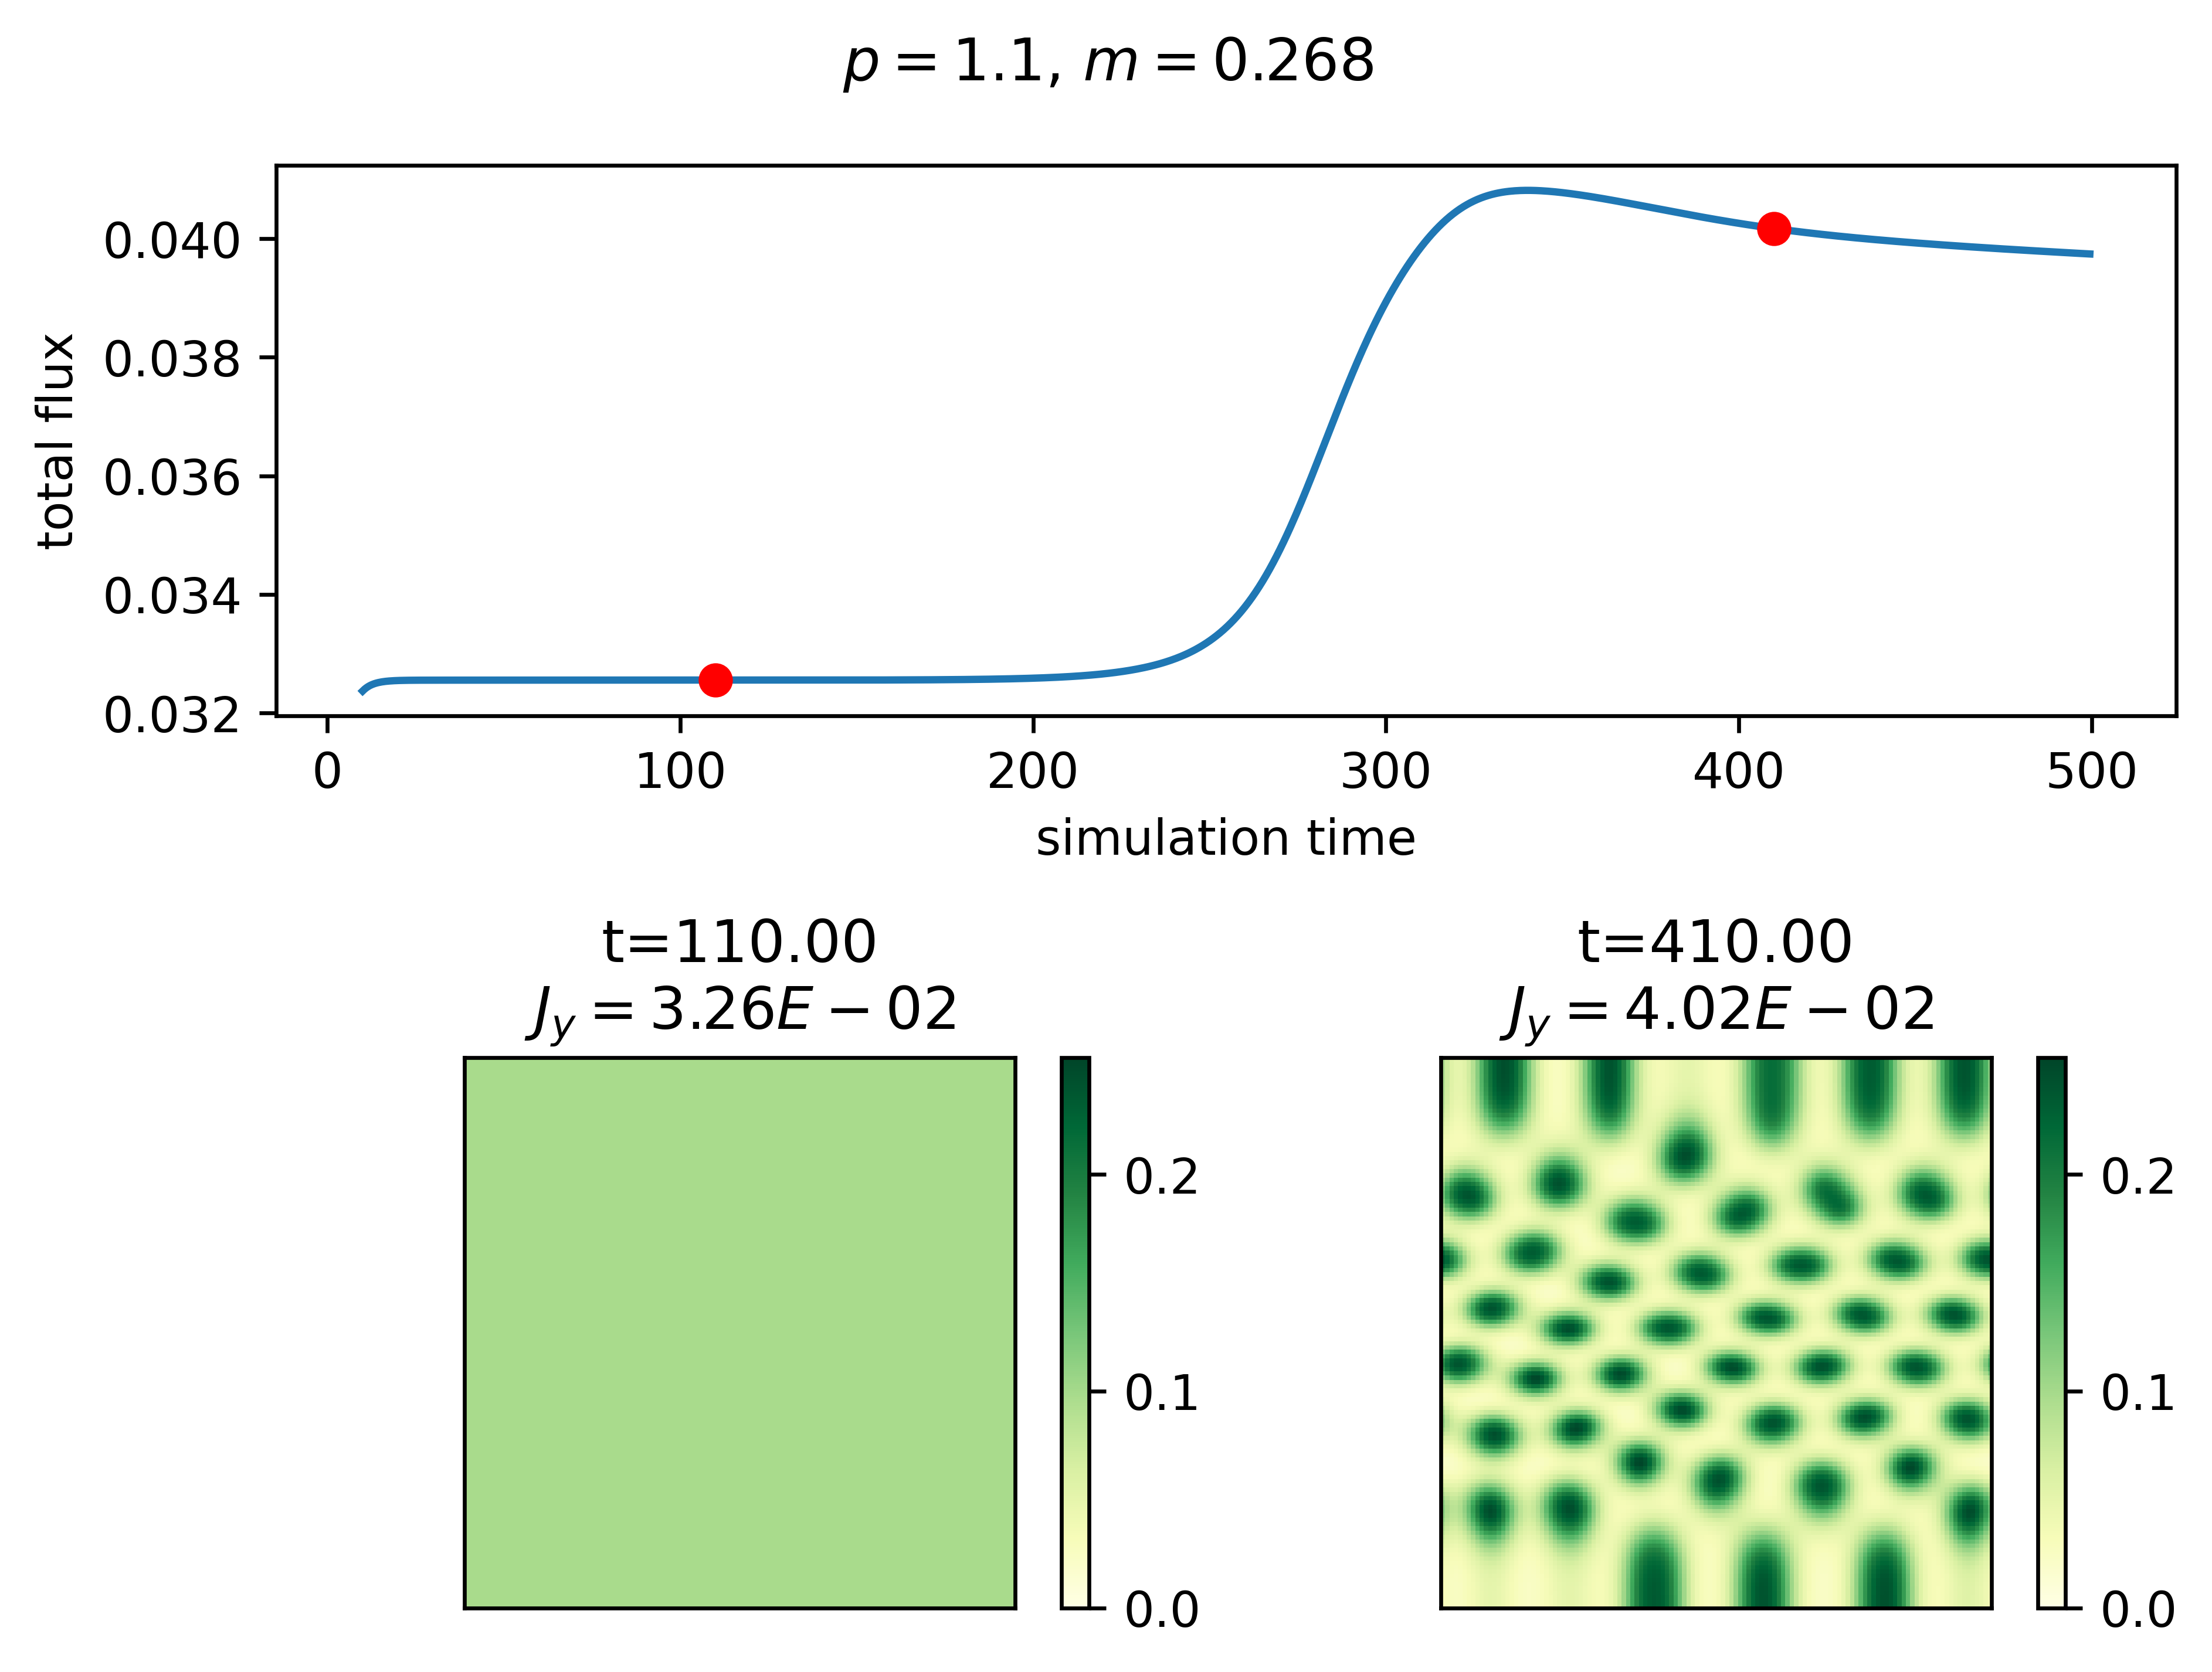
\includegraphics[scale=0.45]{plots/p1_1_m0_268.png}
        \caption{$15^\circ$ slope}
        \label{fig:slope_15}
    \end{subfigure}
    \hskip2em
    \begin{subfigure}{.4\linewidth}
        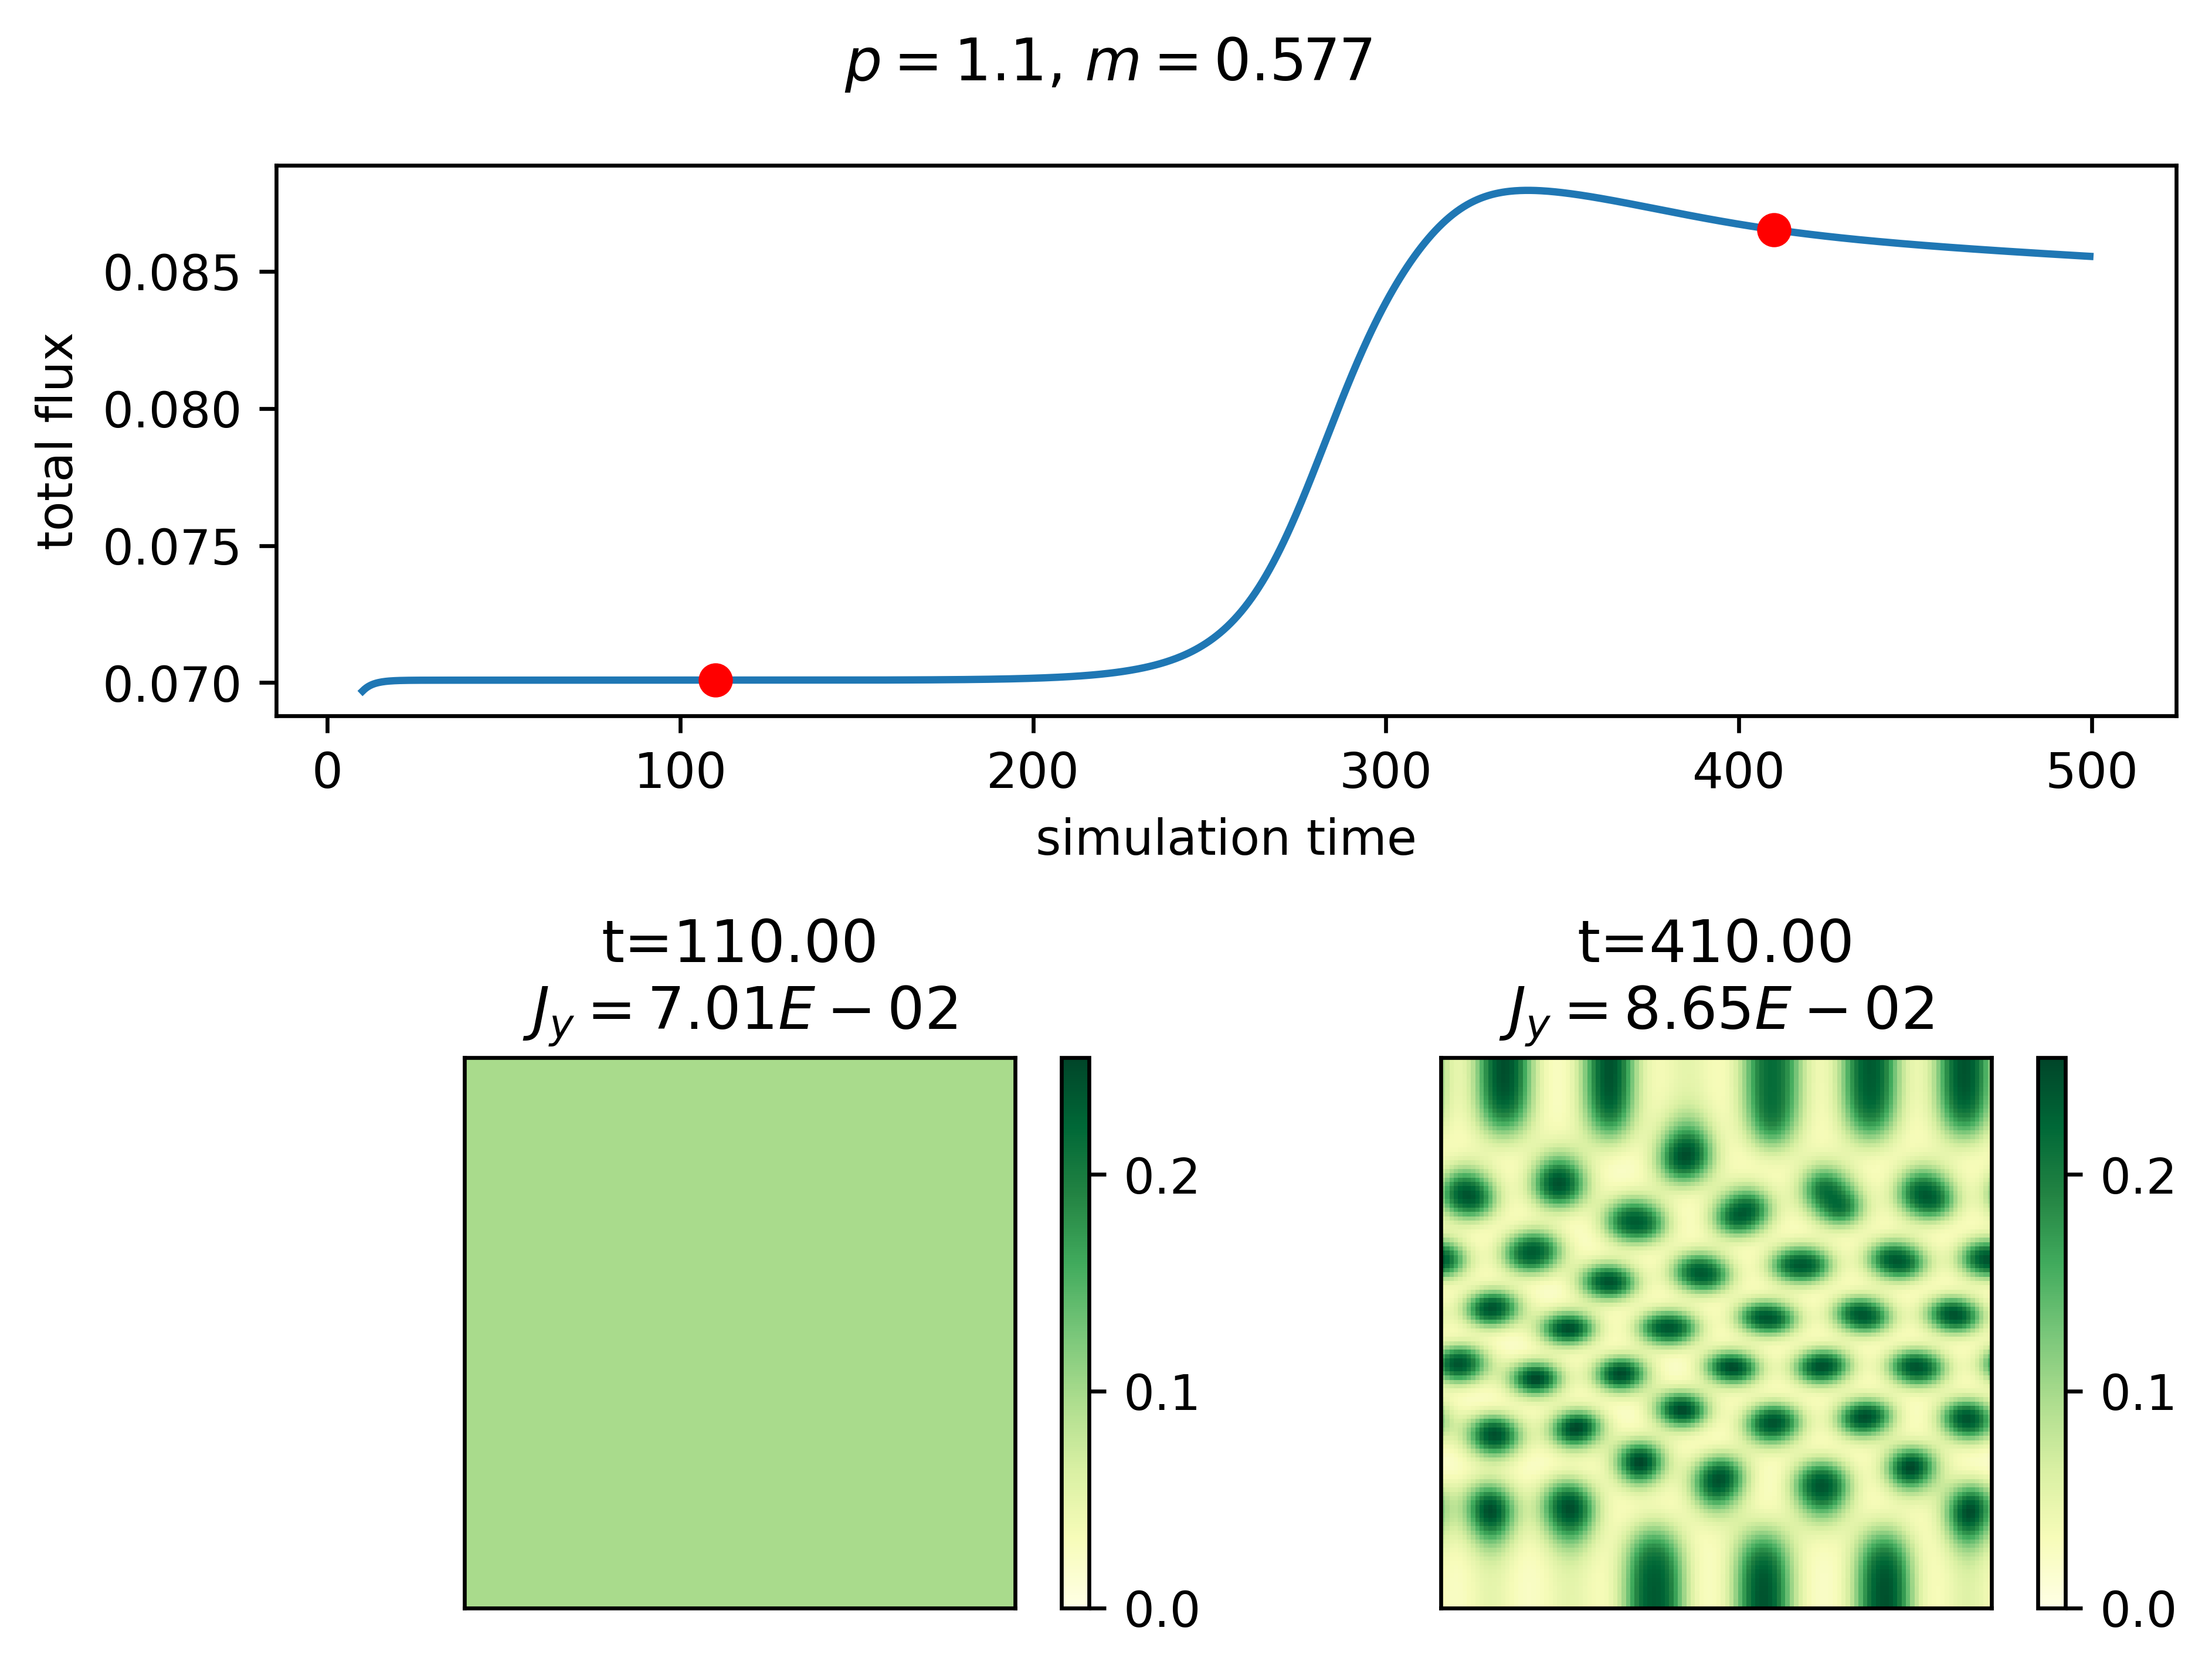
\includegraphics[scale=0.45]{plots/p1_1_m0_577.png}
        \caption{$30^\circ$ slope}
        \label{fig:slope_30}
    \end{subfigure}
    \begin{subfigure}{.4\linewidth}
        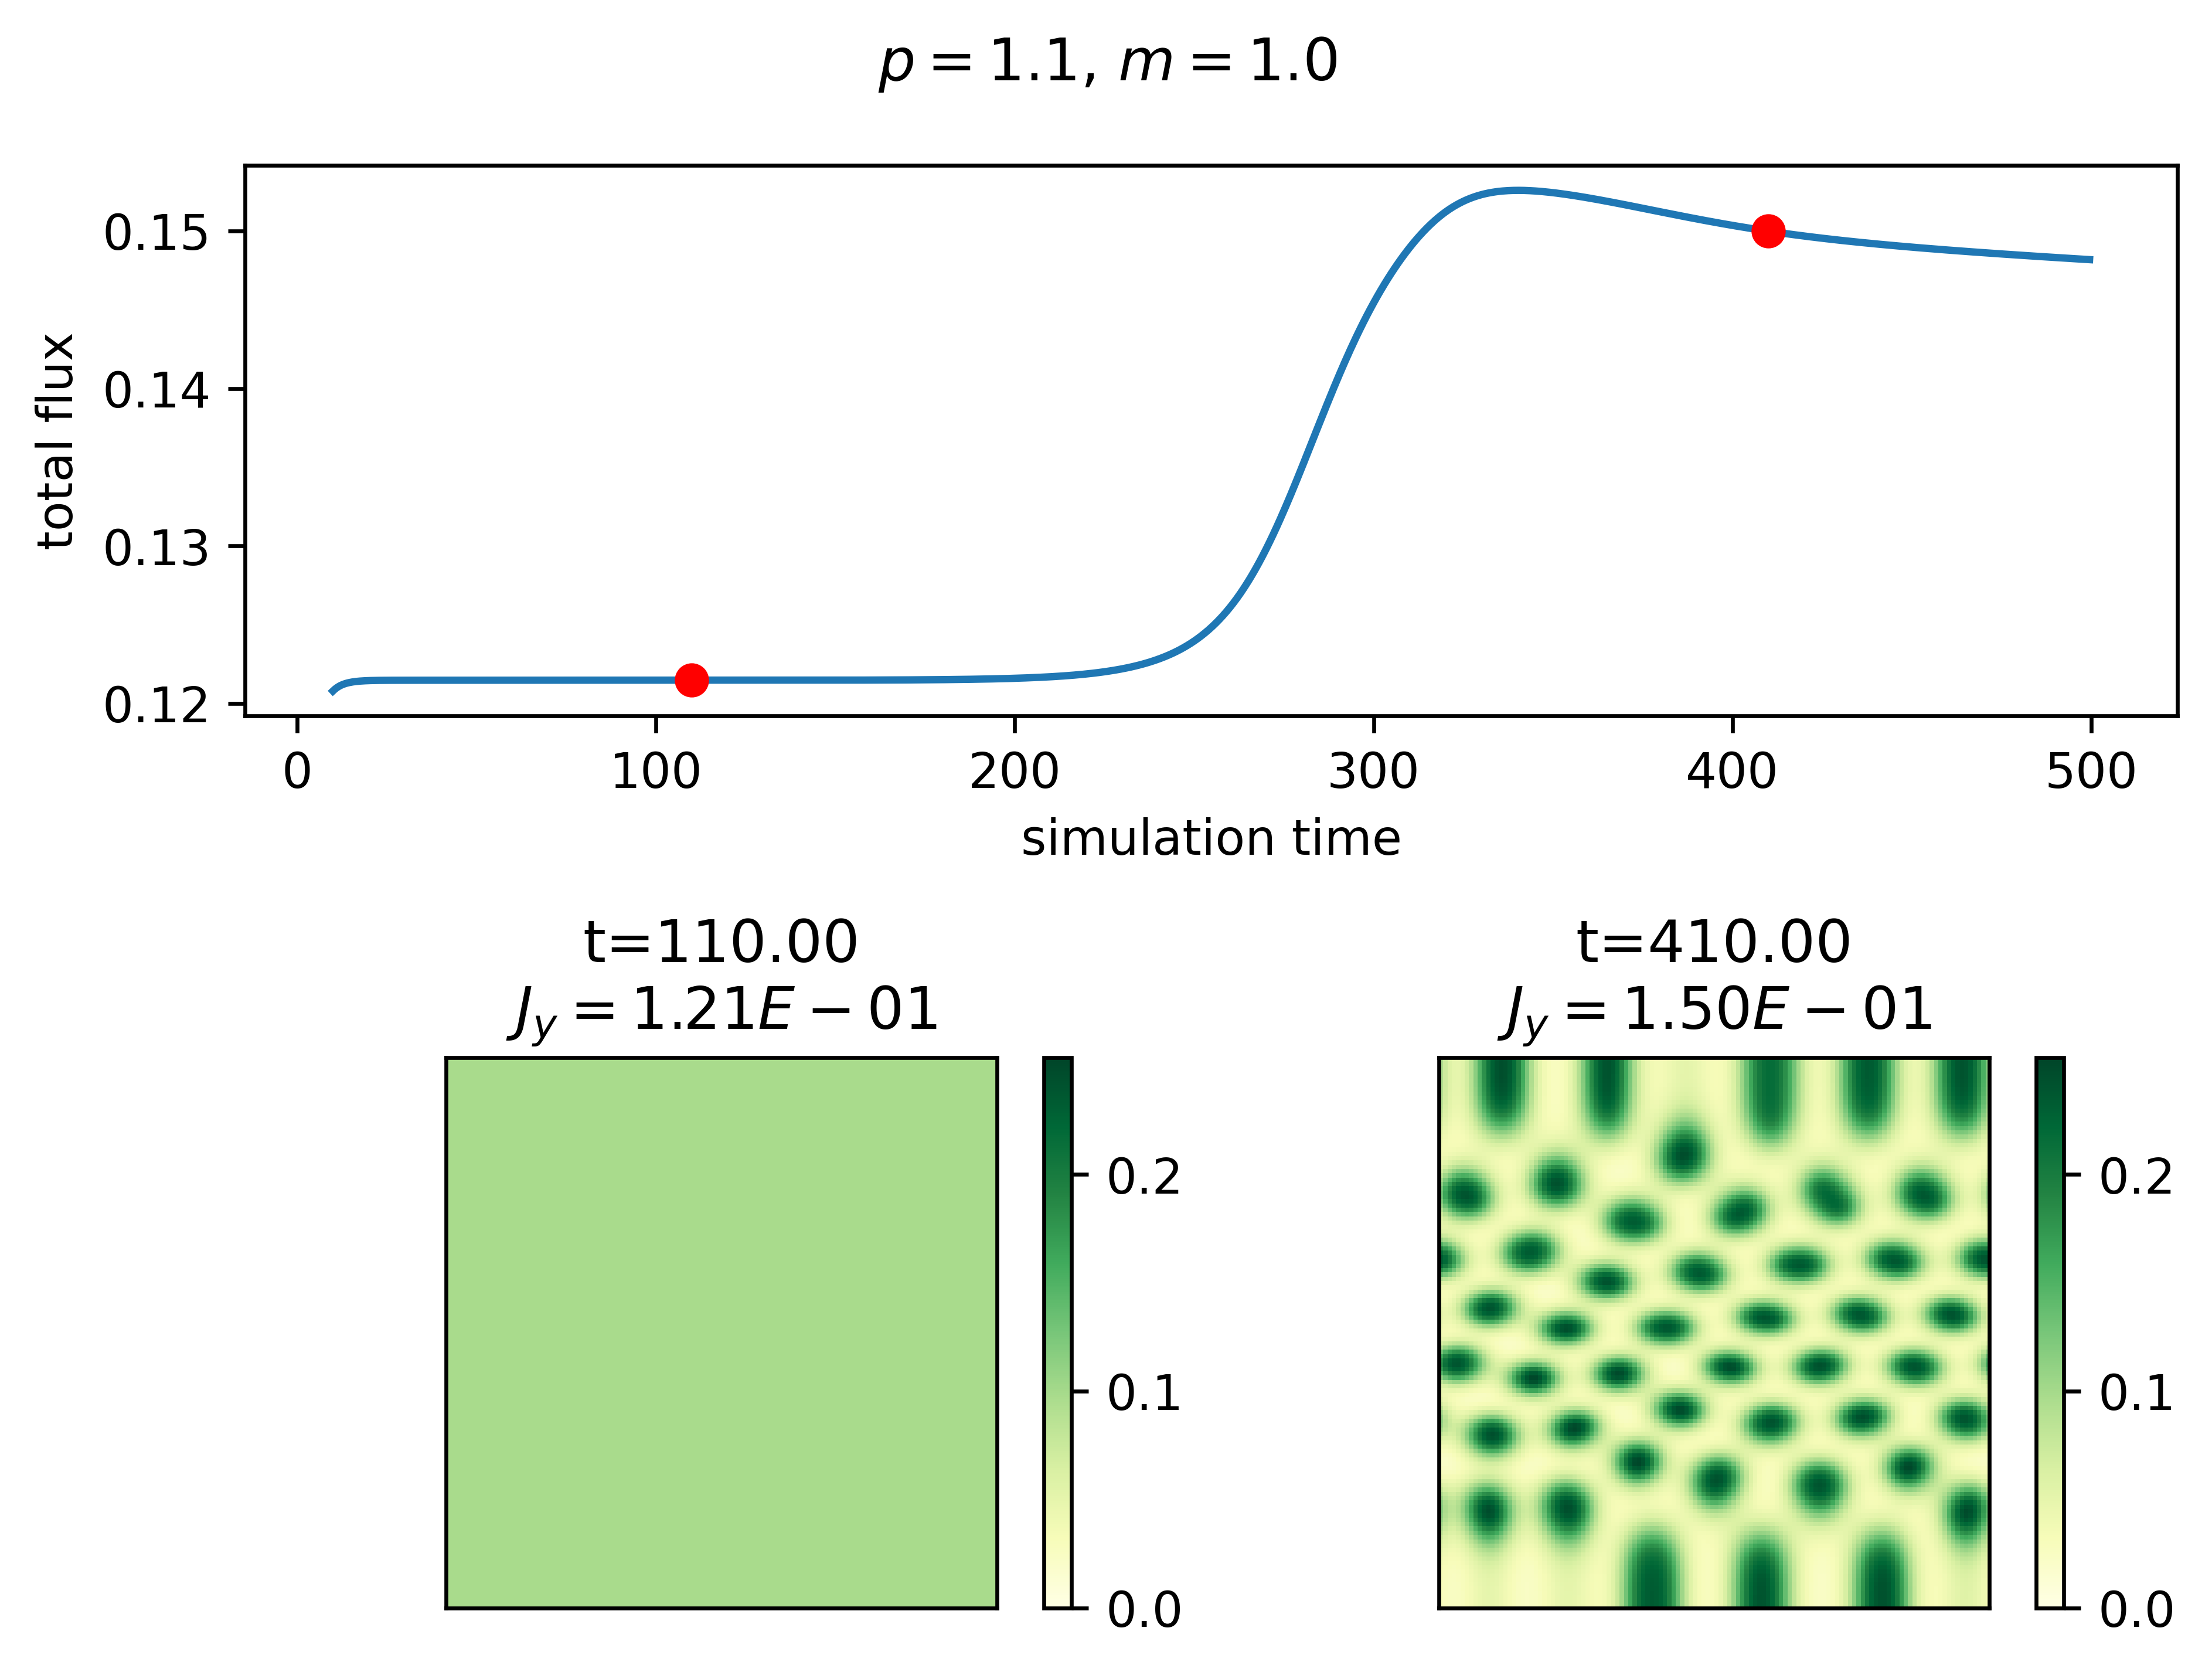
\includegraphics[scale=0.45]{plots/p1_1_m1_0.png}
        \caption{$45^\circ$ slope}
        \label{fig:slope_45}
    \end{subfigure}
    \caption{Simulations of different slopes.}
    \label{fig:flux_out_slopes}
\end{figure}

\begin{figure}[ht!]
    \centering
    \begin{subfigure}{.4\linewidth}
        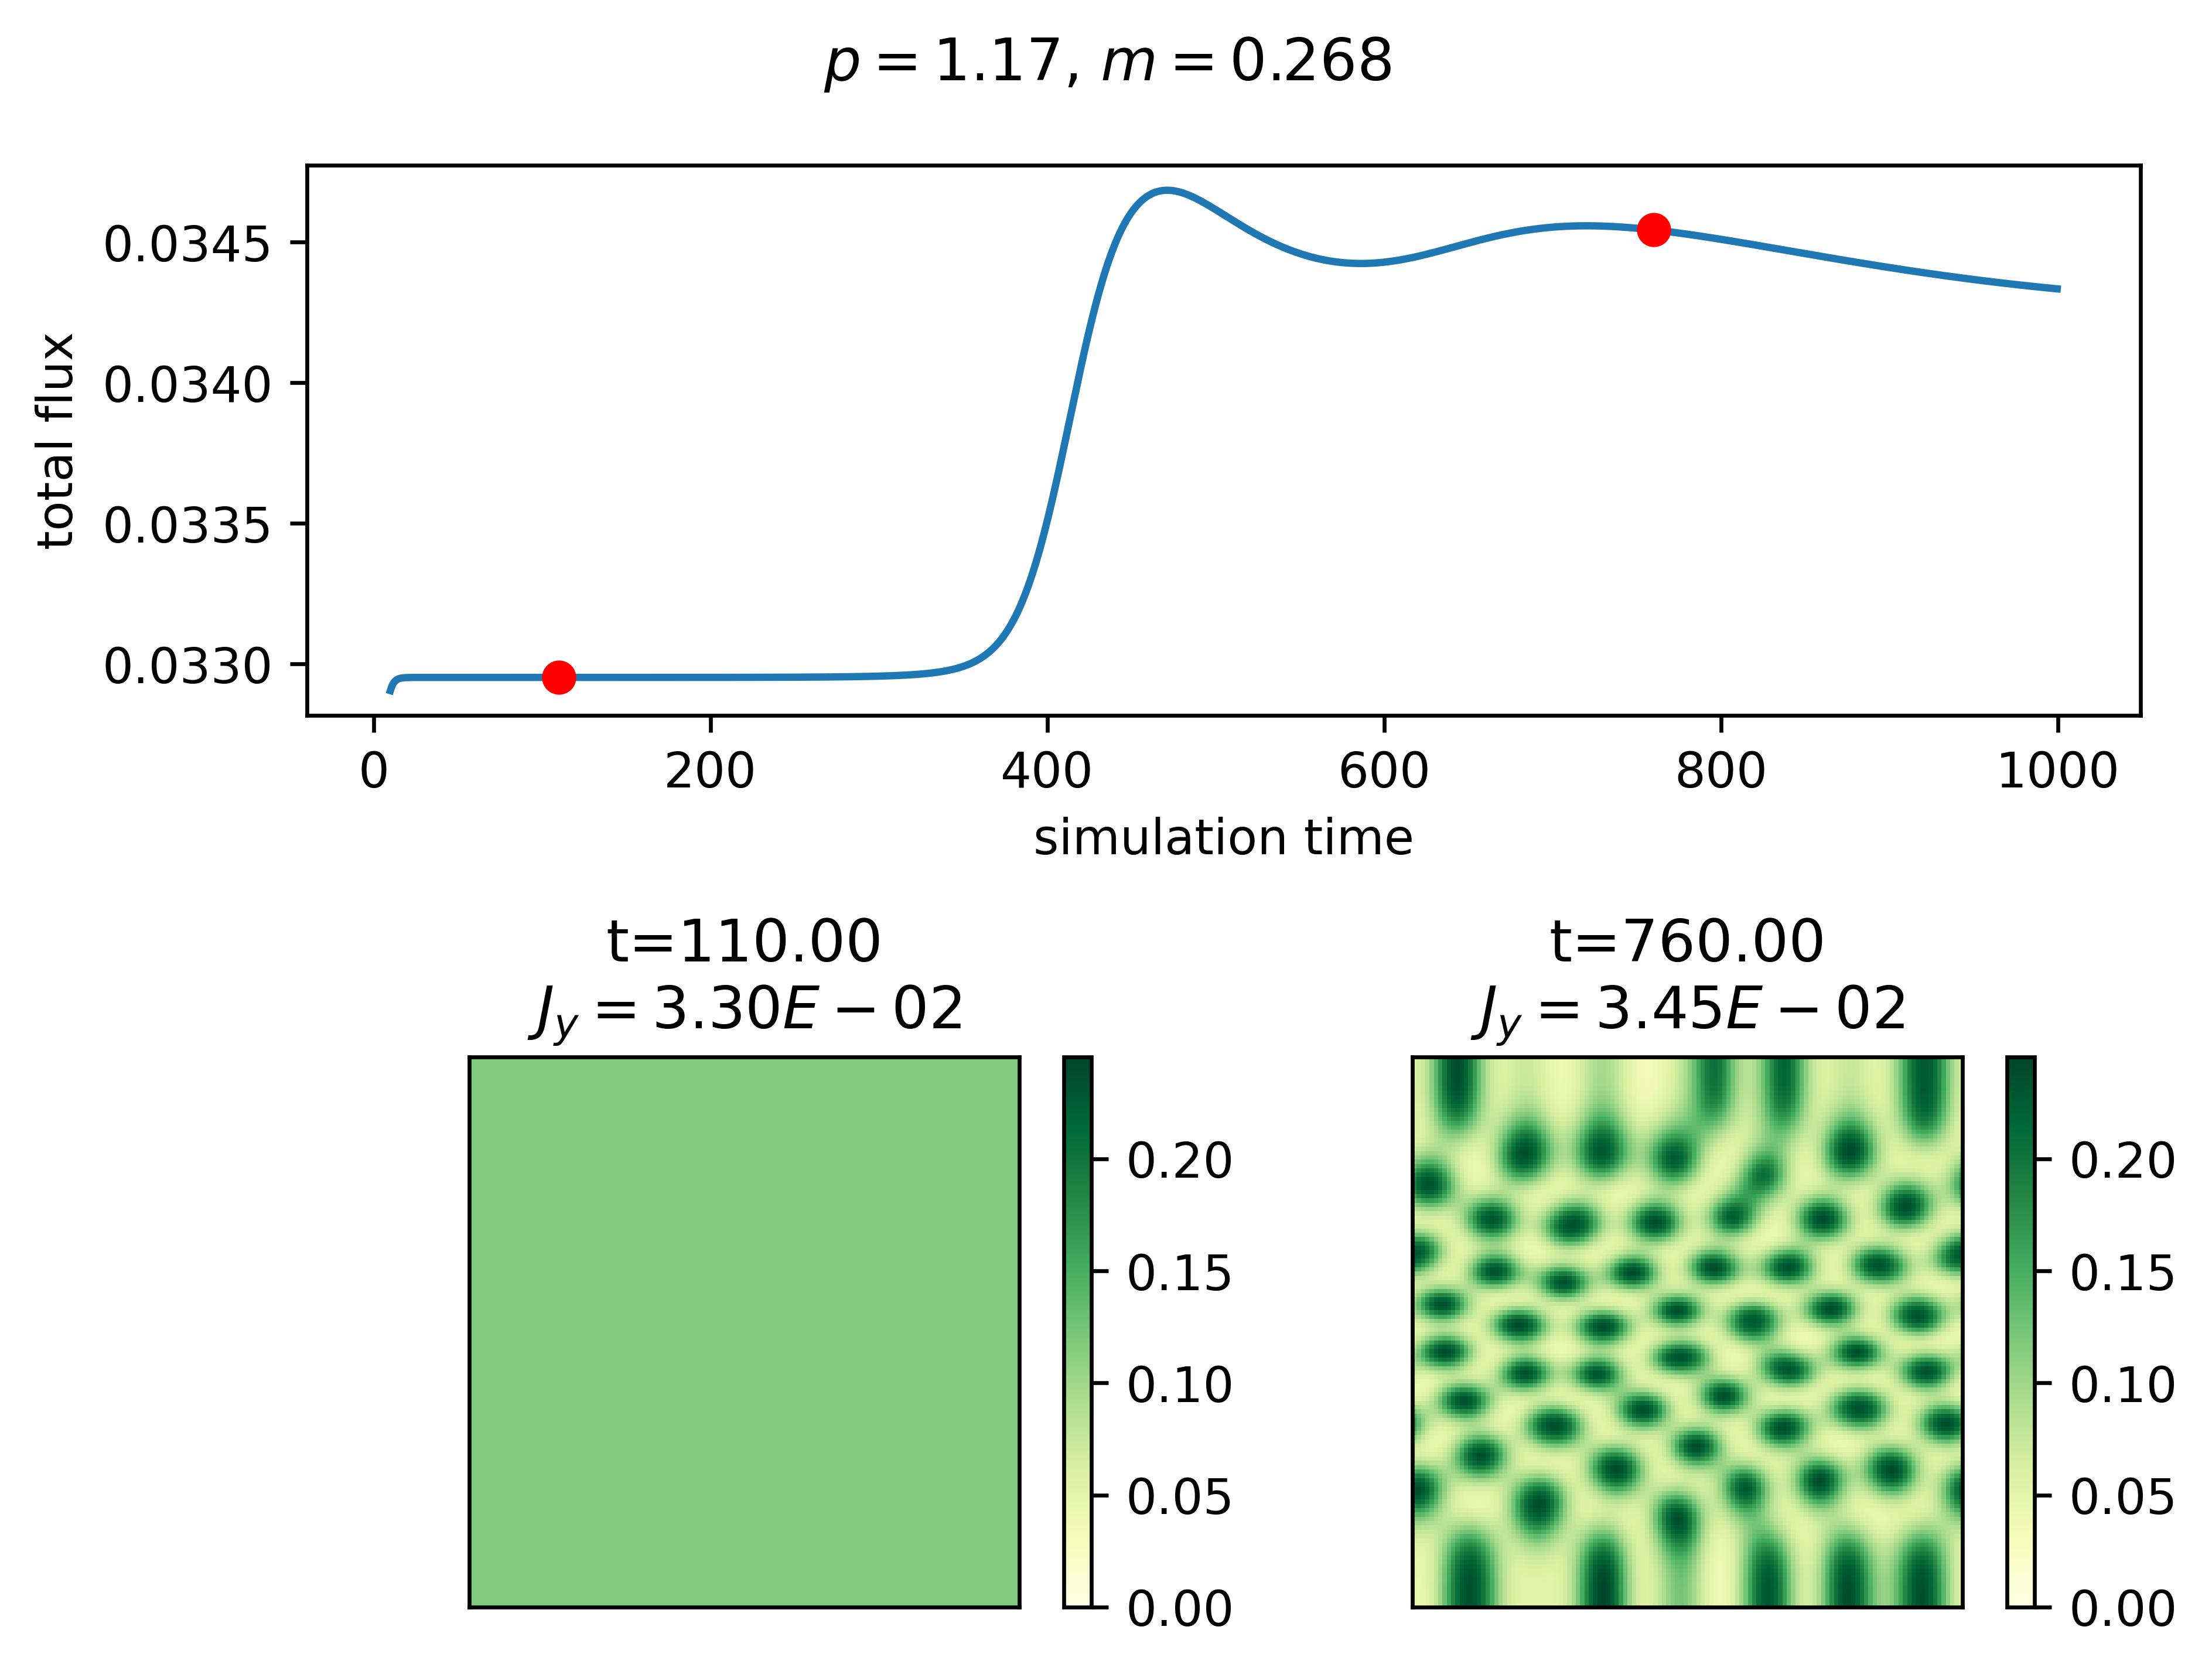
\includegraphics[scale=0.45]{plots/p1_17_m0_268.png}
        \caption{$p=1.17$}
        \label{fig:p_17}
    \end{subfigure}
    \hskip2em
    \begin{subfigure}{.4\linewidth}
        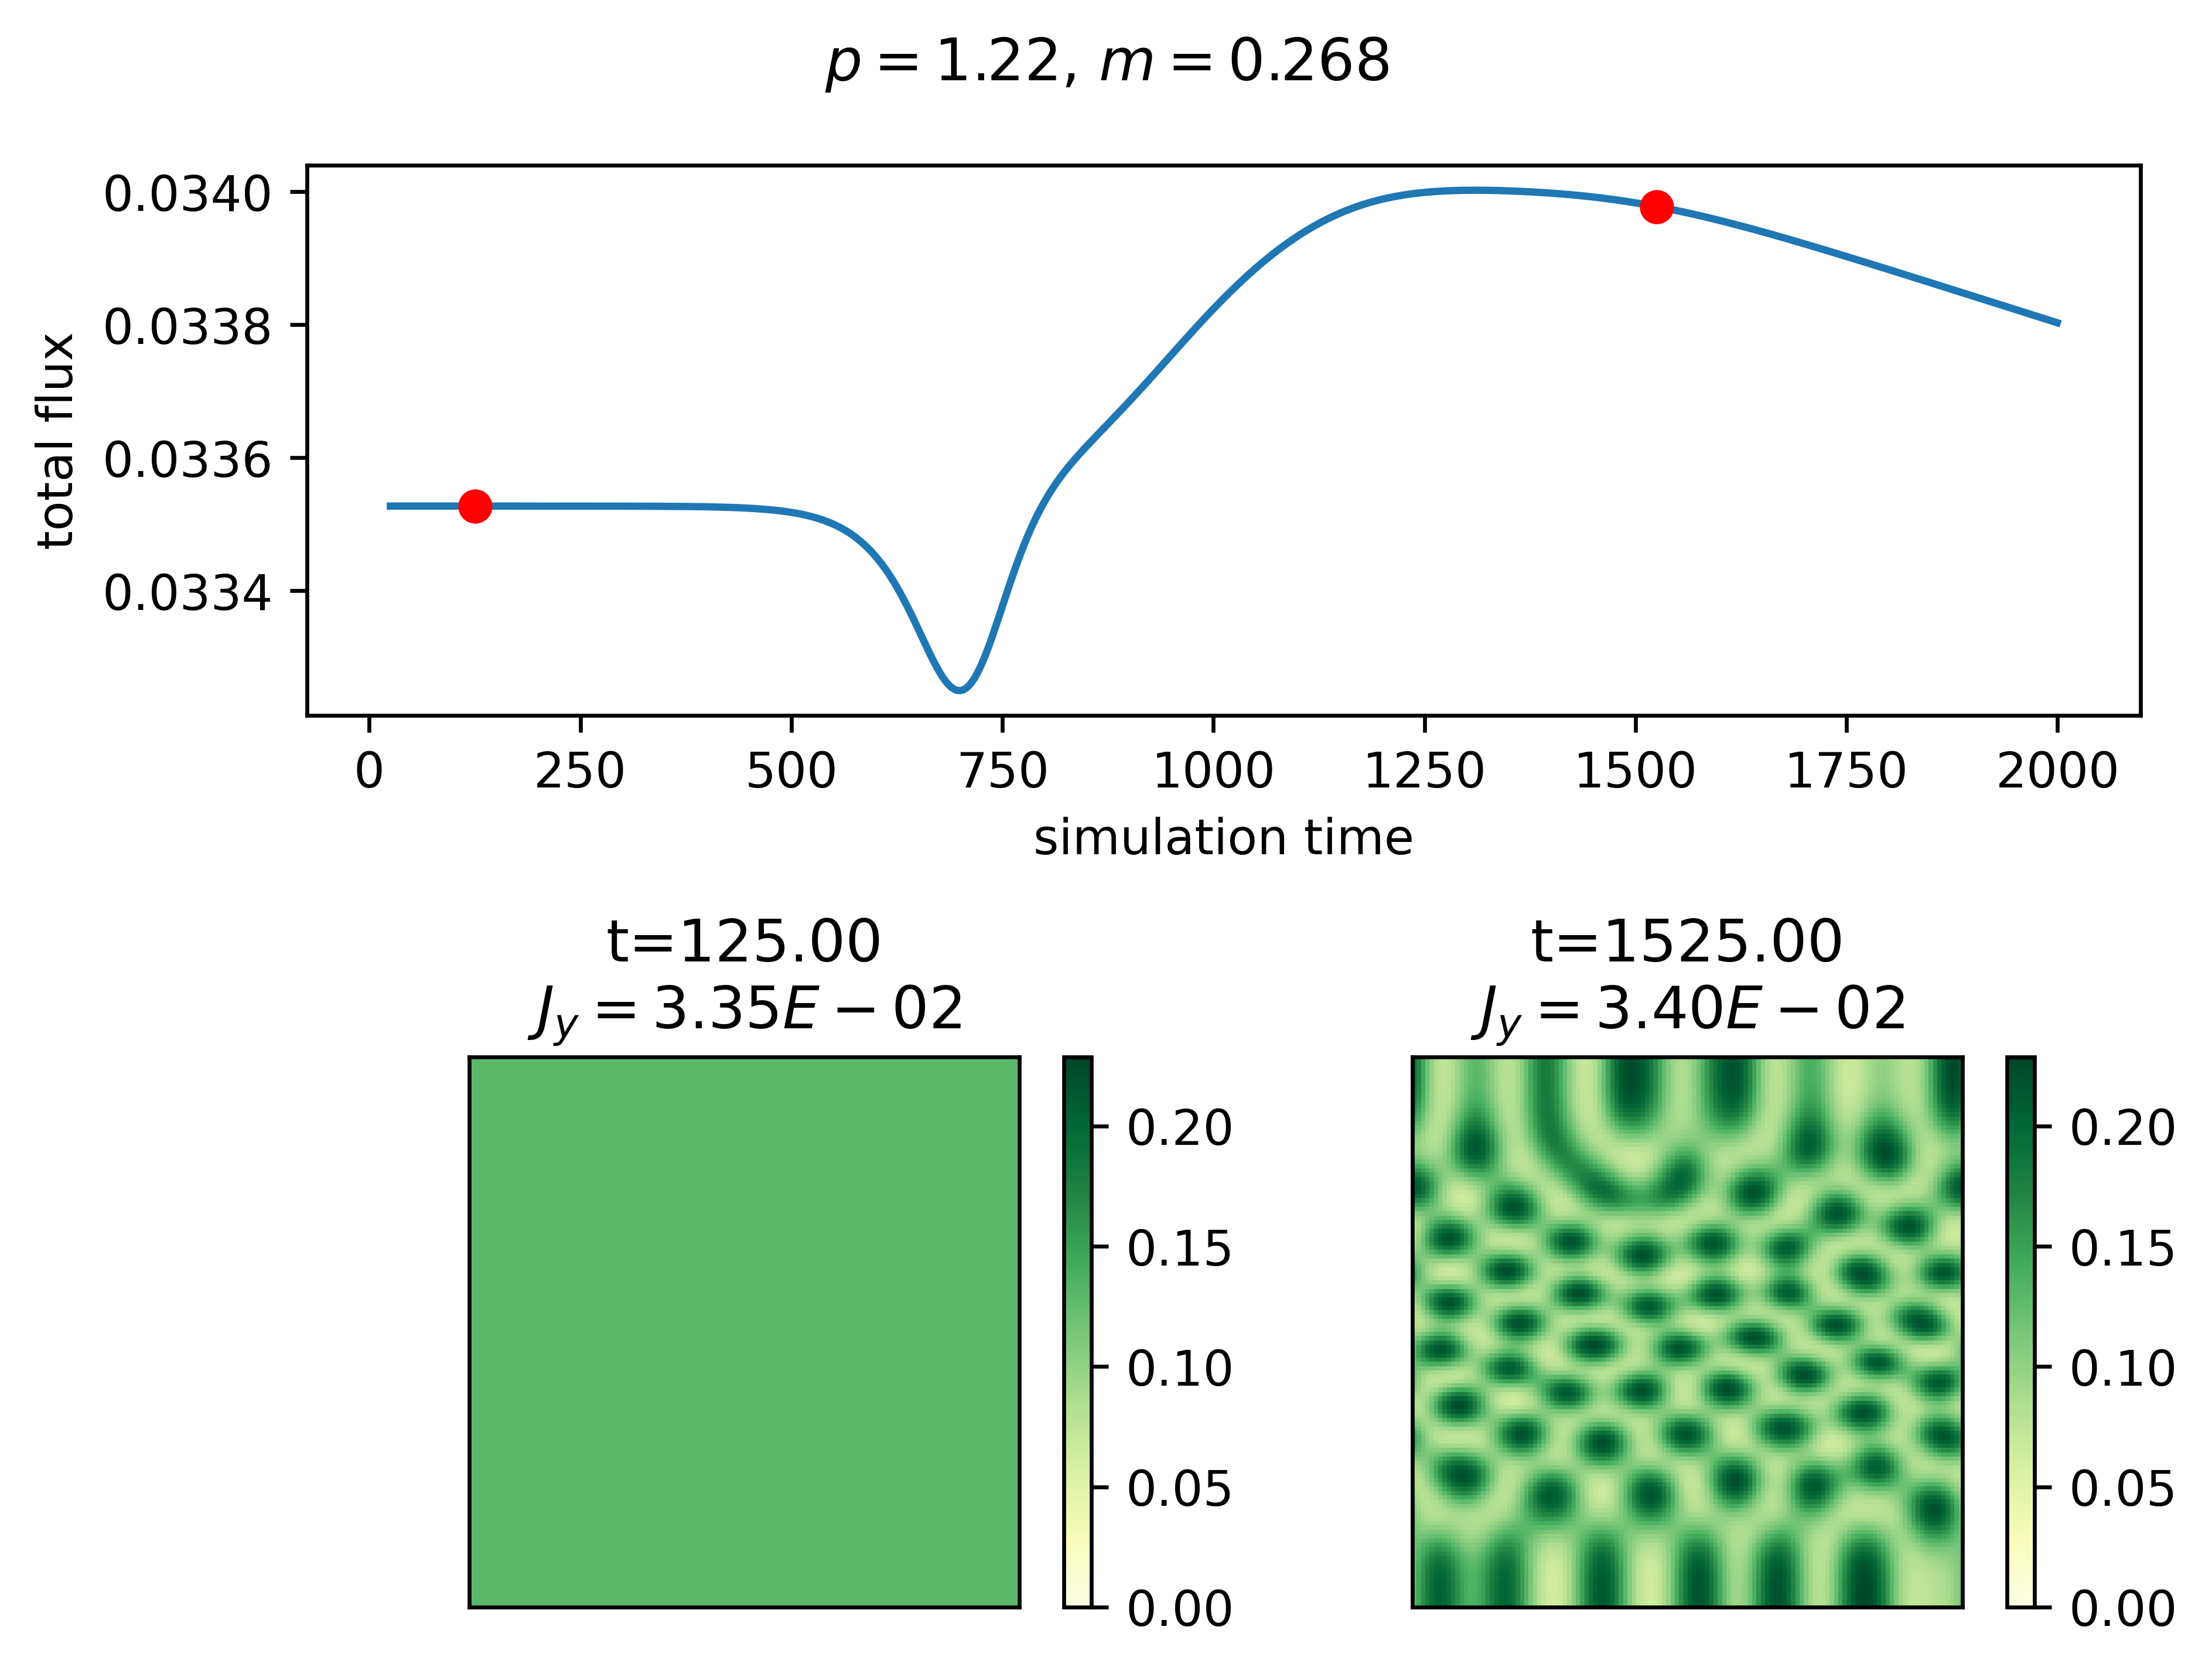
\includegraphics[scale=0.45]{plots/p1_22_m0_268.png}
        \caption{$p=1.22$}
        \label{fig:p1_22}
    \end{subfigure}
    \caption{Simulations of different precipitation values.}
    \label{fig:flux_out_precipitation}
\end{figure}

We also plot the flux on a vertical slice in two time points (figure \ref{fig:flux_slices}).

\begin{figure}[ht!]
    \centering
    \begin{subfigure}{.4\linewidth}
        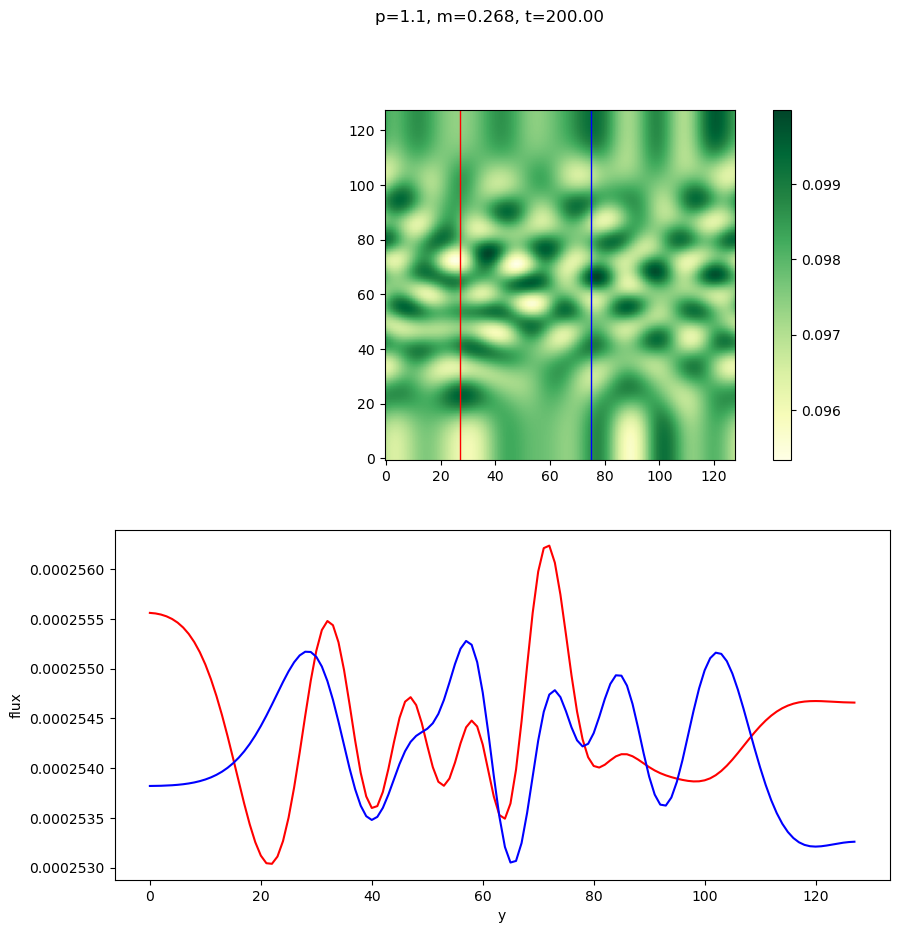
\includegraphics[scale=0.3]{plots/flux_slice_p1_1_m0_268_t200.png}
        \caption{simulation time $t=200$}
        \label{fig:slice_t200}
    \end{subfigure}
    \hskip2em
    \begin{subfigure}{.4\linewidth}
        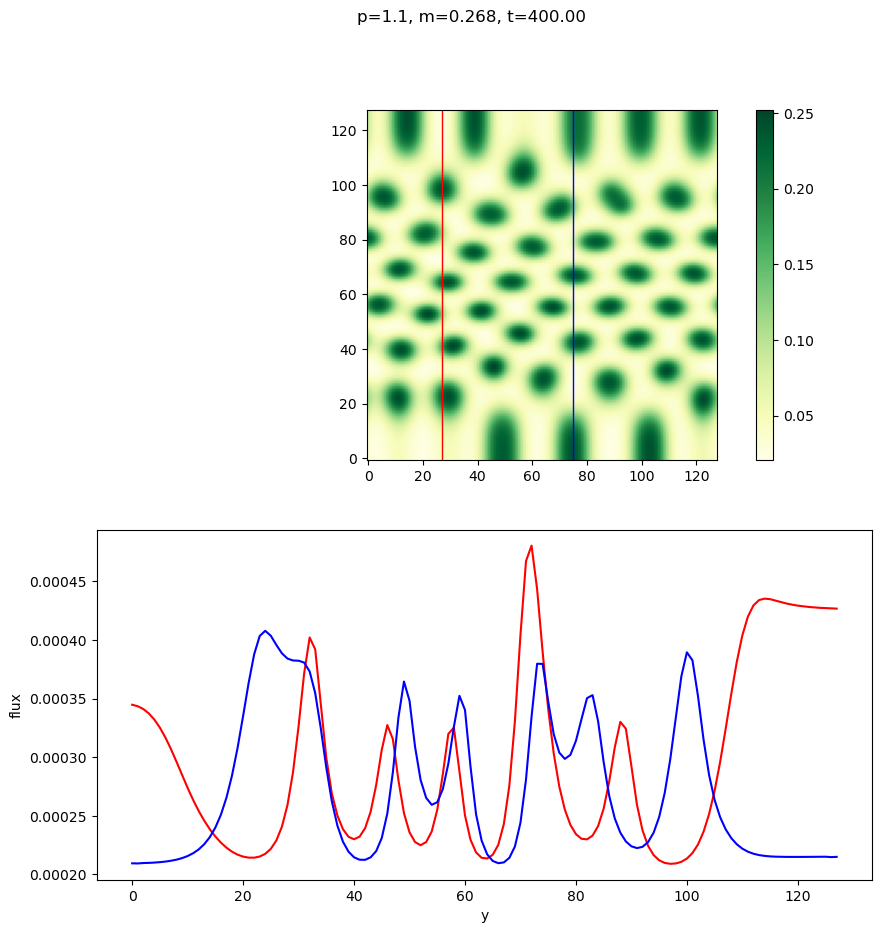
\includegraphics[scale=0.3]{plots/flux_slice_p1_1_m0_268_t400.png}
        \caption{simulation time $t=400$}
        \label{fig:slice_t400}
    \end{subfigure}
    \caption{Water flux in a slice of the region from figure \ref{fig:slope_15}. Each colored plot is the corresponding slice in the simulation.}
    \label{fig:flux_slices}
\end{figure}

\section{Discussion}

Figure \ref{fig:critical_point} Shows that $p_c$ is the critical precipitation in the numerical simulation.
Furthermore, The first mode to grow in the simulations is the uniform vegetation state, which is related to the dispersion curve \ref{eq:sigma1}, where the first mode to grow is the uniform mode, $k=0$.
Those phenomena where anticipated by the model, and assure us that our numerical simulation is correct.

In figure \ref{fig:flux_out_slopes} we see that the change in the slope does not yields a change in the behavior of the system. As was shown in the previous section. The slope is small enough to not effect $\partial_t h$ in the simulations.

In figure \ref{fig:flux_out_precipitation} we see the expected result, that as we increase the precipitation, the final pattern in the simulation is correspond to pattern with higher biomass.
spots patterns becomes stripe patterns, and stripe patterns becomes gap patterns.
Furthermore, we can see the higher the precipitation, the lower the outward flux.
This suggest that patterns that emerge in higher precipitation are better suited to retain water in the system.
We attribute the increased outward water flux to a higher degree of water connectivity in the spots patterns, and to a lesser extent, stripe and gap patterns.
That is to say, water can move farther without being absorbed by the soil or vegetation.

Figure \ref{fig:flux_slices} shows the water flux in a vertical slice of the region. We can see that larger spots correspond to higher flux coming into them, and lower flux coming out of them. In Addition, in figure \ref{fig:slice_t400}, we see that the flux in a single slice is preiodic with the constant amplitude, i.e., the water connectivity is constant in the system. Looking at a transient state of the system, see figure \ref{fig:slice_t200}, we see that the flux is periodic, but the amplitude is not constant. We relate this to different water connectivity in different points in the system.

In regions experiencing droughts or desertification, precipitation levels decrease. Our simulations indicate that this decrease can contribute to an increased outward waterflux. The reduction in precipitation shifts the system to a pattern with less biomass, subsequently leading to enhanced connectivity in the surface water. This increased connectivity manifests as higher outward water flux.

In this study, we have ventured into a relatively unexplored area by applying a mathematical model to understand the relationship between vegetation patterns and water flux in drainage basins. This approach, while different from traditional ecological studies, offers a new lens through which to view and understand these systems.

However, we acknowledge that our study has its limitations. Our simulations are based on certain assumptions and specific conditions, and may not fully capture all real-world scenarios. For example, the impact of human activities on vegetation patterns and water flux was not considered in our model. Future research could aim to incorporate these factors to provide a more nuanced understanding.
Additional research should also take into account periodic precipitation patterns, as we only considered constant precipitation in our simulations.

\section{Bibliography}
\printbibliography

\end{document}
